% 최종 보고서: IDM 전문가 기반 BC와 Anchored PPO를 이용한 노형오거리 자율주행
% XeLaTeX로 컴파일한다(Overleaf: Menu -> Compiler -> XeLaTeX). figures/ 폴더를 함께 올린다.
% 수치 출처: results/final (최종 모델과 평가, git에 포함), results/ablation_envs,
%           results/ablation_lane_penalty, results/ppo_scratch, results/junction_study.
% 주요 평가는 교차로 안 충돌까지 센다(평가 스크립트 기본값).
\documentclass[10pt,a4paper]{article}
\usepackage[margin=2.2cm]{geometry}
\usepackage{kotex}
\usepackage{amsmath,amssymb}
\usepackage{graphicx}
\usepackage{booktabs,tabularx,array,multirow}
\usepackage{algorithm}
\usepackage{algpseudocode}
\usepackage{xcolor}
\usepackage{enumitem}
\usepackage[hidelinks]{hyperref}

\newcolumntype{L}{>{\raggedright\arraybackslash}X}
\newcommand{\Dtr}{\mathcal{D}_{\mathrm{train}}}
\newcommand{\Dval}{\mathcal{D}_{\mathrm{val}}}
\newcommand{\CE}{\mathrm{CE}}
\newcommand{\KL}{D_{\mathrm{KL}}}
\newcommand{\vmax}{v_{\max}}
\algrenewcommand\algorithmicrequire{\textbf{입력:}}
\algrenewcommand\algorithmicensure{\textbf{출력:}}
\floatname{algorithm}{알고리즘}
\renewcommand{\tablename}{표}
\renewcommand{\figurename}{그림}
\setlist{itemsep=1pt, topsep=3pt}

\title{IDM 전문가 데이터를 이용한 행동 복제와 Anchored PPO 기반\\ 노형오거리 자율주행 정책 학습}
\author{}
\date{2026년 11월}

\begin{document}
\maketitle

\begin{abstract}
제주 노형오거리를 재현한 SUMO 환경에서 ego 차량 한 대가 주어진 경로를 신호와 교통을 지키며 끝까지 주행하는 policy를 학습한다.
ego에는 차선 변경 안전 게이트, 속도 상한 같은 규칙 기반 장치를 두지 않으며, 경로를 따르려면 어느 lane에 있어야 하는지는 observation에 넣지 않는다.
SUMO의 IDM 배경 차량을 전문가로 삼아 약 9,876만 개의 상태-행동 쌍을 수집해 행동 복제(BC)로 policy를 초기화하고, BC policy에 KL anchor를 건 PPO(Anchored PPO)로 미세 조정한다.
출발 차선을 무작위로 바꾼 테스트 7,050건에서, 교차로 안 충돌까지 세면 BC는 90.79\%, BC $\rightarrow$ PPO는 97.21\%의 성공률을 보였고, PPO는 빨강 신호 위반을 317건에서 30건으로, wrong lane을 200건에서 83건으로 줄였다.
같은 PPO를 BC 없이 처음부터 학습하면 정지 상태로 수렴해 한 번도 도착하지 못했다.
환경 수, 차선 변경 벌점, 교차로 안 충돌 검사에 대한 추가 실험과 재현성 검증 결과도 함께 보고한다.
\end{abstract}

\section{서론}

\subsection{과제와 목표}
노형오거리(5지 신호 교차로)에서 ego 차량이 24개 경로 중 하나를 받아, 임의의 출발 차선에서 시작해 목적지 도로 끝까지 도착하는 것이 목표다.
실패는 충돌, 빨강 신호 위반, 경로를 벗어난 lane에 갇힘(wrong lane), 시간 초과(500\,s)로 나눈다.

\subsection{제약}
\begin{itemize}
  \item \textbf{규칙 기반 장치 없음.} 학습과 평가 모두 ego의 차선 변경 안전 게이트, 출발 구간 차선 변경 금지, 속도 상한, 교차로 안 차선 변경 금지를 끈다. SUMO의 ego 모드는 \texttt{speedMode 0}, \texttt{laneChangeMode 0}이라 자동 감속과 신호 준수도 없다. Policy가 실행하지 못하는 명령은 없는 lane으로의 변경 같은 물리적으로 불가능한 것뿐이다.
  \item \textbf{경로 lane 정보 금지.} 경로를 완주하려면 어느 lane을 따라야 하는지는 observation에 넣지 않는다(\S\ref{sec:obs}).
\end{itemize}

\subsection{접근}
그림~\ref{fig:overview}처럼 세 단계로 학습한다. (1) SUMO 배경 교통의 IDM 차량을 ego와 같은 방식으로 관측해 전문가 데이터를 만들고, (2) BC로 policy를 학습한 뒤, (3) BC policy를 초기값이자 KL anchor로 삼아 사건 보상으로 PPO를 학습한다.
비교를 위해 BC 단독과 BC $\rightarrow$ PPO를 같은 평가로 보고하고, BC 없이 처음부터 학습한 PPO(PPO 단독)의 결과도 함께 적는다.

\begin{figure}[t]
\centering
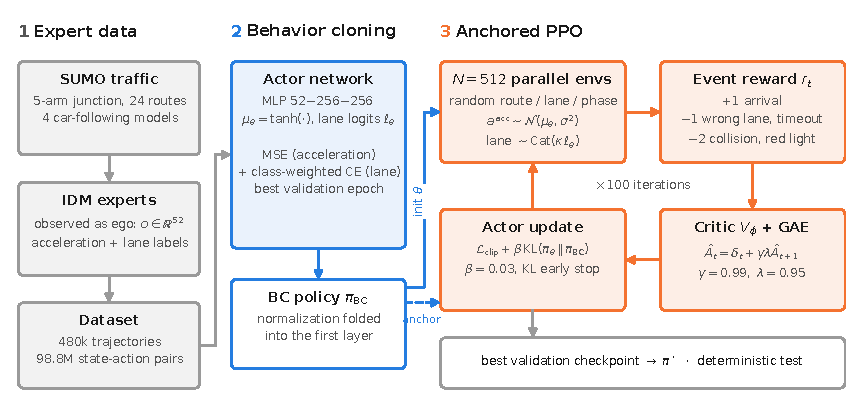
\includegraphics[width=\linewidth]{figures/method_overview.pdf}
\caption{전체 학습 과정. 실선 ``init $\theta$''는 PPO actor를 BC 가중치로 시작한다는 뜻이고, 점선 ``anchor''는 PPO 손실에 BC policy와의 KL을 더한다는 뜻이다. Ego는 규칙 기반 제약 없이 policy 명령을 그대로 실행한다.}
\label{fig:overview}
\end{figure}

\section{환경}

\subsection{도로, 신호, 교통}
\begin{itemize}
  \item \textbf{도로.} 다섯 갈래(A1--A5)가 중앙 신호 교차로에서 만난다. 갈래당 진입 3--5 lane, 진출 2--4 lane이며 제한속도는 13.89\,m/s다. 우회전 샛길(순환도로) 5개와 교차로 앞 유턴(A2, A5)이 있다.
  \item \textbf{신호.} 차선 단위 묶음 신호 5단계, 주기 120\,s: A1·A2 직진(20\,s) $\rightarrow$ A1·A2 좌회전·유턴(17\,s) $\rightarrow$ A3(18\,s) $\rightarrow$ A5(20\,s) $\rightarrow$ A4(20\,s). 단계마다 노랑 3\,s, 전체 빨강 2\,s.
  \item \textbf{배경 교통.} 4,700대/시간, 보정된 출발지-도착지 비율, 포아송 도착. 차종은 Krauss 35\%, IDM 30\%, EIDM 20\%, ACC 15\%이고 속도를 위한 추월은 IDM만 한다. 충돌 판정 간격은 0.2\,m다.
  \item \textbf{충돌 검사.} 평가는 교차로 안 충돌까지 센다(SUMO \texttt{--collision.check-junctions}, 평가 스크립트의 기본값). 전문가 수집과 PPO 학습은 SUMO 기본값(교차로 안은 검사하지 않음)을 쓴다(\S\ref{sec:junction}).
  \item \textbf{Ego.} 가속·감속 한계 5.4\,m/s$^2$, 출발 속도 10\,m/s. 경로는 중앙 교차로 19개와 순환도로 5개, 모두 24개다.
\end{itemize}

\subsection{종료 판정}
Step은 0.5\,s이고 에피소드는 최대 1,000 step(500\,s)이다. 빨강 신호 위반(정지선을 빨강에 통과), 충돌, 도착(경로 끝), wrong lane(경로로 이어지지 않는 lane 끝에서 멈춤, 또는 경로가 아닌 lane으로 교차로에 들어가 제거됨), 시간 초과 순으로 판정한다.

\subsection{평가 세트}\label{sec:suites}
\begin{table}[h]
\centering
\caption{평가 세트. 무작위 출발 차선 세트는 사례마다 SUMO를 새로 시작해(사례별 seed) 결과가 사례 순서와 무관하다.}
\label{tab:suites}
\small
\begin{tabularx}{\linewidth}{@{}lLrl@{}}
\toprule
세트 & 구성 & 사례 & 용도 \\
\midrule
고정 경로 & 24 경로 $\times$ 교통 상태 75개(seed 0), 가운데 lane 출발 & 1,800 & BC 학습 직후 점검 \\
검증 & 94 (경로 $\times$ 출발 lane) $\times$ 교통 상태 30개(seed 62101--62110) & 2,820 & PPO checkpoint 선택 \\
테스트 & 94 $\times$ 교통 상태 75개(seed 52101--52125) & 7,050 & 최종 판단 \\
\bottomrule
\end{tabularx}
\end{table}
고정 경로 세트는 PPO 학습 교통 상태와 같은 실행(seed 0)에서 나와 PPO 평가에는 쓰지 않는다. 검증·테스트 세트는 같은 방식으로 만들되 서로 겹치지 않는 seed를 쓰며, 학습과도 겹치지 않는다. 테스트는 최종 판단에만 쓰고, 설정 선택은 모두 검증으로 한다.

\section{방법}

\subsection{Observation (52차원)}\label{sec:obs}
\begin{table}[h]
\centering
\caption{Observation 구성. 거리는 시야 $W=50$\,m, 속도는 $\vmax=13.89$\,m/s로 나눈다. 자세한 정의는 \texttt{docs/observation\_ko.tex}.}
\label{tab:obs}
\small
\begin{tabularx}{\linewidth}{@{}llL@{}}
\toprule
index & 항목 & 내용 \\
\midrule
0 & ego 속도 & $v/\vmax$ \\
1--20 & 이웃 차량 & lane 5개(왼쪽 둘째 $\sim$ 오른쪽 둘째) $\times$ (leader 간격, 상대속도, follower 간격, 상대속도). lane 연결을 따라 bumper 기준으로 측정 \\
21--25 & lane 연결 & lane이 시야 안에서 끝나는지. 어디로든 이어지면 1(경로는 보지 않음) \\
26--30 & 앞쪽 밀도 & 시야 안 차량 수 / (가용 길이 / 7.5\,m) \\
31--34 & 신호 & 가장 가까운 정지선 신호의 색(one-hot)과 거리(/200\,m) \\
35--42 & 길안내 & 다음 두 갈림길의 거리(/650\,m)와 회전 방향($\sin, \cos$) \\
43--48 & 순환도로 합류 & ring 위 여부, 합류 지점 거리, 본선 차량 2대 \\
49--50 & 길안내 lateral & 나갈 도로 입구 중심과의 좌우 거리(/50\,m) \\
51 & 출발 위치 & 첫 도로에서 $\min(1, s/20\,\mathrm{m})$ \\
\bottomrule
\end{tabularx}
\end{table}
Lane offset은 $k \in (+2, +1, 0, -1, -2)$ 순서이며 $+1$이 왼쪽이다. 기본 31개(index 0--30)만 $[-1,1]$로 clip하고, 입력 정규화(학습 데이터의 평균·표준편차)는 policy 첫 layer에 접어 넣었다. 묶음별 정의는 다음과 같다.

\paragraph{속도 (0).} $o_0 = \operatorname{clip}(v/\vmax)$. 제한속도에서 1로 포화되므로 그보다 빠른 속도는 구분하지 못한다.

\paragraph{이웃 차량 (1--20).} Lane offset $k$마다 leader와 follower 하나씩을 $\big(g^{\mathrm{lead}}_k/W,\ \operatorname{clip}\tfrac{v^{\mathrm{lead}}_k-v}{\vmax},\ -g^{\mathrm{fol}}_k/W,\ \operatorname{clip}\tfrac{v^{\mathrm{fol}}_k-v}{\vmax}\big)$로 넣는다. 간격은 bumper 기준($g^{\mathrm{lead}} = \Delta s - \ell_{\mathrm{lead}}$, $g^{\mathrm{fol}} = -\Delta s - \ell_{\mathrm{ego}}$)이며, lane 연결을 따라 앞으로 $W+5$\,m, 뒤로 $W+{}$ego 길이까지 찾는다. 연결된 모든 lane을 보고 경로로 거르지 않는다. 옆 lane은 겹치면 음수가 되도록 부호를 유지하고, 현재 lane은 0 이상으로 자른다. 차량이 없으면 leader $(1,1)$, follower $(-1,-1)$이다.

\paragraph{Lane 연결 (21--25).} Lane $k$의 남은 길이를 $r_k$라 할 때 $c_k = -1$(lane 없음), $1$($r_k > W$ 또는 lane에서 나가는 link가 하나라도 있음), $r_k/W$(그 밖)이다. 교차로 안에서는 1이다. ``어디로든 이어지는가''만 보며, 경로와 맞는지 확인하는 함수는 observation에서 호출되지 않는다(\texttt{tests/test\_bc\_observation.py}가 검사).

\paragraph{앞쪽 밀도 (26--30).} $\rho_k = \operatorname{clip}_{[0,1]}\big(n_k / (L_k/7.5\,\mathrm{m})\big)$. 가용 길이 $L_k$는 lane이 이어지면 $W$, 막다른 lane이면 $\min(W, r_k)$이고, lane이 시야 안에서 끝나면 첫 번째 연결 lane(경로와 무관)의 차량도 센다. Lane이 없으면 1, 교차로 안에서는 0이다.

\paragraph{신호 (31--34).} Ego가 지날 연결의 가장 가까운 정지선 신호를 (빨강, 노랑, 초록) one-hot과 정지선 거리 $d_{\mathrm{stop}}/200$\,m로 넣는다. 100\,m 밖이거나 신호가 없으면 0이다.

\paragraph{길안내 (35--42, 49--50).} 나가는 도로가 둘 이상인 도로 선택 지점(이 도로망에 29개) 중 경로상 다음 두 곳을 $\big(1,\ d_i/650\,\mathrm{m},\ \sin\Delta\psi_i,\ \cos\Delta\psi_i\big)$로 넣는다. $d_i$는 주행 거리, $\Delta\psi_i$는 들어오는 도로 끝과 나가는 도로 시작의 heading 차이다($\sin>0$이면 좌회전). Lateral(49--50)은 나갈 도로의 \emph{모든} lane 시작점 중심과 ego의 좌우 거리 $e_i/50$\,m다. 어느 \emph{도로}로 갈지만 알려 주고 어느 \emph{lane}인지는 알려 주지 않는다. 다만 회전 방향과 lateral은 어느 쪽으로 가야 하는지를 간접적으로 알려 준다.

\paragraph{순환도로 합류 (43--48).} Ego가 ring lane에 있을 때만 값이 생긴다: ring 위 여부, 합류 지점까지 주행 거리($/50$\,m, 없으면 $-1$), 합류 지점 50\,m 안의 본선 차량 2대의 (속도$/\vmax$, 거리$/50$\,m)(없으면 $(0,-1)$).

\paragraph{출발 위치 (51).} 첫 도로에서 $\min(1, s/20\,\mathrm{m})$, 이후 1. IDM 전문가는 수집 때 첫 도로 20\,m 안에서 lane 변경이 막혀 있었으므로, policy가 그 구간을 볼 수 있게 넣었다. Ego에는 그런 제한이 없다.

\paragraph{넣지 않는 것.} 경로를 따르려면 어느 lane에 있어야 하는지(목적지 lane, lookahead connectivity)는 넣지 않는다. 또한 교차로 안에서 경로가 겹치는 상충 차량, 없는 lane과 빈 lane의 구분(이웃 칸에서는 둘 다 $(1,1,-1,-1)$)은 observation에 없다.

\subsection{Action}
Action은 $[u_{\mathrm{acc}}, u_{\mathrm{lane}}] \in [-1,1]^2$이다. 가감속은 $a = 5.4\,u_{\mathrm{acc}}$\,m/s$^2$이고 목표 속도 $\max(0, v + 0.5a)$를 지정한다. Lane 명령은 $u_{\mathrm{lane}} \ge 0.5$면 왼쪽, $\le -0.5$면 오른쪽, 그 사이면 유지다. Policy 출력은 가감속 평균 $\mu=\tanh(\cdot)$와 lane logit 3개이며, 평가는 $\mu$와 argmax로 결정적으로 행동한다.

\subsection{IDM 전문가 데이터}
\begin{itemize}
  \item 새 SUMO 시뮬레이션을 3,600\,s씩 2,268회 실행했다(12 프로세스, 1.76시간). 20회 중 1회는 검증 실행으로 나눴다(학습 2,155 / 검증 113).
  \item 각 실행에서 \texttt{car\_idm} 배경 차량을 하나씩 잠시 ego로 놓고 ego와 같은 코드로 observation을 계산한다. 가감속 label은 $(v_{t+1}-v_t)/(0.5\,\mathrm{s}\times 5.4\,\mathrm{m/s^2})$, lane label은 SUMO의 lane 변경 기록이다.
  \item 닫힌 IDM 궤적 309만 개 중, 경로마다 학습 19,000개와 검증 1,000개를 출발 시각 세 구간에 고르게 골라 48만 궤적을 만들었다.
  \item 표본은 9,876만 쌍(학습 9,381만 / 검증 495만)이다. Lane 변경 label은 학습 표본의 0.73\%뿐이다.
  \item IDM 전문가는 수집 때 첫 도로 20\,m 안에서 lane 변경이 막혀 있었다. Ego에는 이 제한이 없고, 대신 observation 51번으로 그 구간을 볼 수 있다.
\end{itemize}

\subsection{BC와 Anchored PPO}
알고리즘~\ref{alg:bc-ko}와 \ref{alg:ppo-ko}에 전체 절차를, 표~\ref{tab:hparams-ko}에 하이퍼파라미터를 정리했다.
BC는 가감속 MSE와 class 가중 cross entropy(lane)를 줄인다. Lane class 가중치는 빈도의 역수에 1/4 거듭제곱을 취해 평균 1로 맞춘 값이다(왼쪽 1.317, 유지 0.329, 오른쪽 1.353).
PPO는 BC actor로 시작하고, 손실에 $\beta\,\KL(\pi_\theta \| \pi_{\mathrm{BC}})$를 더해 BC policy에서 크게 벗어나지 않게 한다.
BC 단계는 보상을 쓰지 않는다. PPO는 기존 형성 보상(shaped reward, \texttt{train.py}의 \texttt{REWARD})을 모두 버리고, 표~\ref{tab:reward}의 사건 보상과 lane 변경 벌점($c = 0.01$, \S\ref{sec:penalty})만 쓴다.
\[
r_t = -10^{-4} - c\,\mathbb{1}[\text{lane 변경 실행}] + \begin{cases}
+1 & \text{도착} \\
-1 & \text{wrong lane 또는 시간 초과} \\
-2 & \text{충돌 또는 빨강 신호 위반} \\
b_t & \text{그 밖 (빨강 신호 앞 정지 보너스 } 0.01\,e^{-|e|}\text{, 대부분 0)}
\end{cases}
\]

\begin{table}[h]
\centering
\caption{PPO 보상. 한 step에 여러 사건이 겹치면 충돌, 빨강 신호, 도착, wrong lane, 시간 초과 순으로 하나만 준다.}
\label{tab:reward}
\small
\begin{tabularx}{\linewidth}{@{}lrL@{}}
\toprule
항목 & 값 & 조건 \\
\midrule
매 step & $-10^{-4}$ & 항상 \\
도착 & $+1$ & 경로 마지막 도로 끝에 도착 (종료) \\
wrong lane & $-1$ & 경로로 이어지지 않는 lane 끝 5\,m 안에서 0.5\,m/s 미만으로 멈춤, 또는 경로가 아닌 lane으로 교차로에 들어가 SUMO가 ego를 제거 (종료) \\
시간 초과 & $-1$ & 500\,s 안에 끝나지 않음. 실패로 보고 종료 처리(value로 이어 붙이지 않음) \\
충돌 & $-2$ & ego가 충돌 목록에 있음 (종료) \\
빨강 신호 위반 & $-2$ & 빨강 신호일 때 정지선을 통과 (종료) \\
정지 보너스 & $0.01\,e^{-|e|}$ & 빨강 신호가 보이고, 그 step에 lane 변경 명령이 없고, ego가 0.1\,m/s 이하로 그 이동의 lane에 서 있고, 앞 대기열도 멈춰 있을 때 신호당 한 번. $e$는 목표 위치(정지선 1\,m 앞, 또는 멈춘 앞차 뒤 2\,m)와의 거리(m) \\
\midrule
과속 벌점 & 0 (꺼짐) & 정의: $c\,\max(0, v - 1.1\,v_{\mathrm{lim}})/v_{\mathrm{lim}}$ \\
lane 변경 벌점 & $-0.01$ & 실제로 실행된 lane 변경 1회당(없는 lane으로의 명령처럼 실행되지 않은 것은 제외). 최종 모델에 사용(\S\ref{sec:penalty}) \\
\bottomrule
\end{tabularx}
\end{table}

보상의 크기는 결과(도착 $+1$, 실패 $-1$ 또는 $-2$)가 대부분을 차지하도록 잡았다. 에피소드 약 200 step의 step 비용 합은 약 $-0.02$, 정지 보너스는 신호당 최대 $0.01$이라 결과를 뒤집지 않는다. 충돌과 신호 위반을 wrong lane보다 크게 벌해, 안전을 경로 완주보다 우선하게 했다.

\begin{algorithm}[t]
\caption{전문가 데이터 수집과 행동 복제(BC)}
\label{alg:bc-ko}
\begin{algorithmic}[1]
\Require 배경 교통이 있는 SUMO 도로, 전문가로 쓸 IDM 차량, 경로별 할당량 $q_{\mathrm{tr}}, q_{\mathrm{val}}$
\Ensure 원래 관측을 입력받는 BC 정책 $\pi_{\mathrm{BC}}$
\Statex \textit{전문가 수집}
\Repeat
  \State 새 시뮬레이션을 3{,}600\,s 실행한다. 확률 $1/20$로 검증 실행, 나머지는 학습 실행으로 정한다
  \For{닫힌 IDM 궤적의 각 step $t$}
    \State $o_t \gets$ 그 차량을 ego로 놓고 계산한 52차원 관측
    \State $a^{\mathrm{acc}}_t \gets (v_{t+1}-v_t)/(\Delta t\, a_{\max})$,\quad $y_t \gets$ SUMO 차선 변경 $\in\{+1,0,-1\}$
    \State $|a^{\mathrm{acc}}_t|\le 1$이고 $v_{t+1}\le v_{\mathrm{lim}}$이면 $(o_t, a^{\mathrm{acc}}_t, y_t)$를 남긴다
  \EndFor
\Until{모든 경로에서 학습 궤적 $q_{\mathrm{tr}}$개 이상, 검증 궤적 $q_{\mathrm{val}}$개 이상}
\State 경로마다 궤적 단위로 고르되, 출발 시각 세 구간에 고르게 나눈다 $\Rightarrow \Dtr, \Dval$
\Statex \textit{행동 복제}
\State $m_x, \sigma_x \gets \Dtr$에서 구한 관측 특성별 평균과 표준편차
\State $c\in\{\text{왼쪽},\text{유지},\text{오른쪽}\}$마다 $w_c \gets (N/(3 n_c))^{1/r}$, 그 뒤 $\tfrac13\sum_c w_c = 1$이 되도록 나눈다
\State actor $\pi_\theta$ 초기화: MLP $52\!\to\!256\!\to\!256$ (ReLU), 출력 $\mu_\theta=\tanh(\cdot)$와 차선 로짓 $\ell_\theta\in\mathbb{R}^3$
\For{epoch $=1,\dots,E$}
  \For{$\Dtr$의 크기 $B$ 미니배치 $\mathcal{B}$마다}
    \State $\displaystyle \mathcal{L}_{\mathrm{BC}} = \frac{1}{|\mathcal{B}|}\sum_{i\in\mathcal{B}}\big(\mu_\theta(\bar o_i)-a^{\mathrm{acc}}_i\big)^2
      + \frac{\sum_{i} w_{y_i}\,\CE(\ell_\theta(\bar o_i), y_i)}{\sum_{i} w_{y_i}}$, \quad $\bar o = (o-m_x)/\sigma_x$
    \State $\theta \gets \mathrm{Adam}(\theta, \nabla_\theta \mathcal{L}_{\mathrm{BC}})$ \Comment{기울기 노름 1로 제한}
  \EndFor
  \State $\Dval$에서 $\mathcal{L}_{\mathrm{BC}}$를 재고, 가장 낮은 $\theta_{\mathrm{BC}}$를 남긴다
\EndFor
\State 정규화를 첫 층에 접어 넣는다: $W_1 \gets W_1\,\mathrm{diag}(1/\sigma_x)$, $b_1 \gets b_1 - W_1 m_x$
\State \Return $\pi_{\mathrm{BC}} = \pi_{\theta_{\mathrm{BC}}}$
\end{algorithmic}
\end{algorithm}

\begin{algorithm}[t]
\caption{BC 정책에서 시작하는 Anchored PPO 미세 조정}
\label{alg:ppo-ko}
\begin{algorithmic}[1]
\Require $\pi_{\mathrm{BC}}$, 병렬 환경 $N$개, 사건 보상 $r_t$, 표~\ref{tab:hparams-ko}의 하이퍼파라미터
\Ensure 미세 조정된 정책 $\pi_{\theta^\star}$
\State $\theta \gets \theta_{\mathrm{BC}}$, 차선 출력에 $\kappa$를 곱한다: $\ell_\theta \gets \kappa\,\ell_\theta$ \Comment{argmax는 그대로, 표본의 차선 변경은 드물게}
\State 가감속 정책 $\mathcal{N}(\mu_\theta(s), \sigma^2)$, $\sigma$는 학습되며 $\sigma \gets \sigma_0$에서 시작
\State 고정된 기준 정책 $\pi_{\mathrm{anc}} \gets \pi_\theta$ \Comment{차선 출력을 날카롭게 한 BC 정책}
\State critic $V_\phi$ 초기화 (별도 MLP, 입력은 $m_x,\sigma_x$로 표준화)
\For{반복 $k=1,\dots,K$}
  \State 환경 $N$개에서 $\pi_\theta$로 $T$ step씩 주행한다. 에피소드마다 경로, 출발 차선, 신호 위상을 무작위로 정한다
  \State $(s_t, a_t, \log\pi_{\mathrm{old}}(a_t\mid s_t), r_t, d_t)$를 저장한다. $a_t = (a^{\mathrm{acc}}_t, a^{\mathrm{lane}}_t)$
  \State $\delta_t = r_t + \gamma(1-d_t)V_\phi(s_{t+1}) - V_\phi(s_t)$,\quad $\hat A_t = \delta_t + \gamma\lambda(1-d_t)\hat A_{t+1}$,\quad $R_t = \hat A_t + V_\phi(s_t)$
  \State $\hat A$를 배치 전체에서 평균 0, 표준편차 1로 정규화한다
  \For{epoch $=1,\dots,K_V$} \Comment{critic, 매 반복}
    \For{미니배치 $\mathcal{M}$마다} \State $\phi \gets \mathrm{Adam}\big(\phi, \nabla_\phi \tfrac{1}{|\mathcal{M}|}\sum (V_\phi(s)-R)^2\big)$ \EndFor
  \EndFor
  \If{$k > K_{\mathrm{warm}}$} \Comment{critic 예열 뒤 actor}
    \For{epoch $=1,\dots,K_\pi$}
      \For{미니배치 $\mathcal{M}$마다}
        \State $\rho = \pi_\theta(a\mid s)/\pi_{\mathrm{old}}(a\mid s)$, $\log\pi = \log\mathcal{N}(a^{\mathrm{acc}};\mu_\theta,\sigma^2) + \log\mathrm{softmax}(\ell_\theta)_{a^{\mathrm{lane}}}$
        \If{$\frac{1}{|\mathcal{M}|}\sum(\rho - 1 - \log\rho) > 1.5\,\delta_{\mathrm{KL}}$} 이 반복의 actor 업데이트를 \textbf{멈춘다} \EndIf
        \State $\displaystyle \mathcal{L}_{\mathrm{clip}} = -\frac{1}{|\mathcal{M}|}\sum \min\!\big(\rho\hat A,\ \mathrm{clip}(\rho,1-\epsilon,1+\epsilon)\hat A\big)$
        \State $\displaystyle \mathcal{L}_{\mathrm{anc}} = \frac{1}{|\mathcal{M}|}\sum\Big[\frac{(\mu_\theta-\mu_{\mathrm{anc}})^2}{2\sigma_0^2} + \KL\big(\pi^{\mathrm{lane}}_\theta\,\|\,\pi^{\mathrm{lane}}_{\mathrm{anc}}\big)\Big]$
        \State $\mathcal{L}_\pi = \mathcal{L}_{\mathrm{clip}} + \beta\,\mathcal{L}_{\mathrm{anc}}$ \Comment{엔트로피 항 없음}
        \State $\theta \gets \mathrm{Adam}(\theta, \nabla_\theta \mathcal{L}_\pi)$ \Comment{기울기 노름 0.5로 제한}
      \EndFor
    \EndFor
  \EndIf
\EndFor
\State $\theta^\star \gets$ 저장한 체크포인트 중 검증 세트 성공률이 가장 높은 것 (같으면 뒤의 반복)
\State \Return $\pi_{\theta^\star}$ \Comment{평가는 결정적으로: $a^{\mathrm{acc}} = \mu$, $a^{\mathrm{lane}} = \arg\max \ell$}
\end{algorithmic}
\end{algorithm}

\begin{table}[t]
\centering
\caption{알고리즘~\ref{alg:bc-ko}, \ref{alg:ppo-ko}의 하이퍼파라미터.}
\label{tab:hparams-ko}
\begin{tabular}{@{}llll@{}}
\toprule
\multicolumn{2}{@{}l}{행동 복제} & \multicolumn{2}{l}{Anchored PPO} \\
\midrule
경로별 할당량 $q_{\mathrm{tr}}, q_{\mathrm{val}}$ & 19{,}000, 1{,}000 & 환경 수 $N$ / rollout $T$ & 512 / 64 \\
차선 가중치 근 $r$ & 4 & 반복 $K$ / critic 예열 $K_{\mathrm{warm}}$ & 100 / 5 \\
최적화, 학습률 & Adam, $4.2\times10^{-4}$ & actor / critic epoch $K_\pi$ / $K_V$ & 5 / 10 \\
배치 크기 $B$ & 8{,}192 & 미니배치 크기 & 1{,}024 \\
epoch $E$ & 100 & actor / critic 학습률 & $5\times10^{-5}$ / $3\times10^{-4}$ \\
step $\Delta t$, $a_{\max}$ & 0.5\,s, 5.4\,m/s$^2$ & $\gamma$ / $\lambda$ / clip $\epsilon$ & 0.99 / 0.95 / 0.2 \\
관측 / 행동 차원 & 52 / 2 & 기준 계수 $\beta$ / $\sigma_0$ / $\kappa$ & 0.03 / 0.05 / 2 \\
 & & 목표 KL $\delta_{\mathrm{KL}}$ & 0.01 \\
 & & 보상: 도착 / 차선 이탈, 시간 초과 & $+1$ / $-1$ \\
 & & 보상: 충돌, 빨강 신호 위반 / 매 step & $-2$ / $-10^{-4}$ \\
 & & 빨강 신호 앞 정지 보너스 (신호당 한 번) & $0.01\,e^{-|e|}$, $e$는 m \\
 & & lane 변경 벌점 $c$ (실행 1회당) & 0.01 \\
\bottomrule
\end{tabular}
\end{table}

\subsection{PPO 단독}\label{sec:scratch}
BC의 효과를 보기 위해 같은 PPO를 BC 없이 처음부터 학습했다. Actor는 무작위로 초기화하고(입력 정규화만 데이터 평균·표준편차로 맞춤) anchor는 두지 않았다($\beta = 0$). Lane 유지 확률 0.9에서 시작하고, 가감속 탐색 $\sigma=0.5$, 학습률 $3\times10^{-4}$, lane 변경 벌점 0.01을 썼다. 보상과 환경 512개, 나머지 하이퍼파라미터는 BC $\rightarrow$ PPO와 같다.

\subsection{병렬 학습}
PPO는 환경 512개를 SUMO 프로세스 16개에 나눠 돌린다. 프로세스 하나는 도로망을 32벌 복제해 한 시뮬레이션에 넣고(복제본 사이 100\,m 간격, 서로 연결 없음), 복제본마다 ego와 배경 교통을 따로 돌린다(그림~\ref{fig:replicas}). 반복당 $512 \times 64 = 32{,}768$ 전이를 모으고, 100회 학습에 9.4분이 걸렸다(GPU 1개). 작업자 수에 따른 반복당 시간은 4개 13.5\,s, 8개 7.9\,s, 16개 5.5\,s였고, GPU 사용률은 1--3\%로 SUMO 계산이 병목이다.

\begin{figure}[t]
\centering
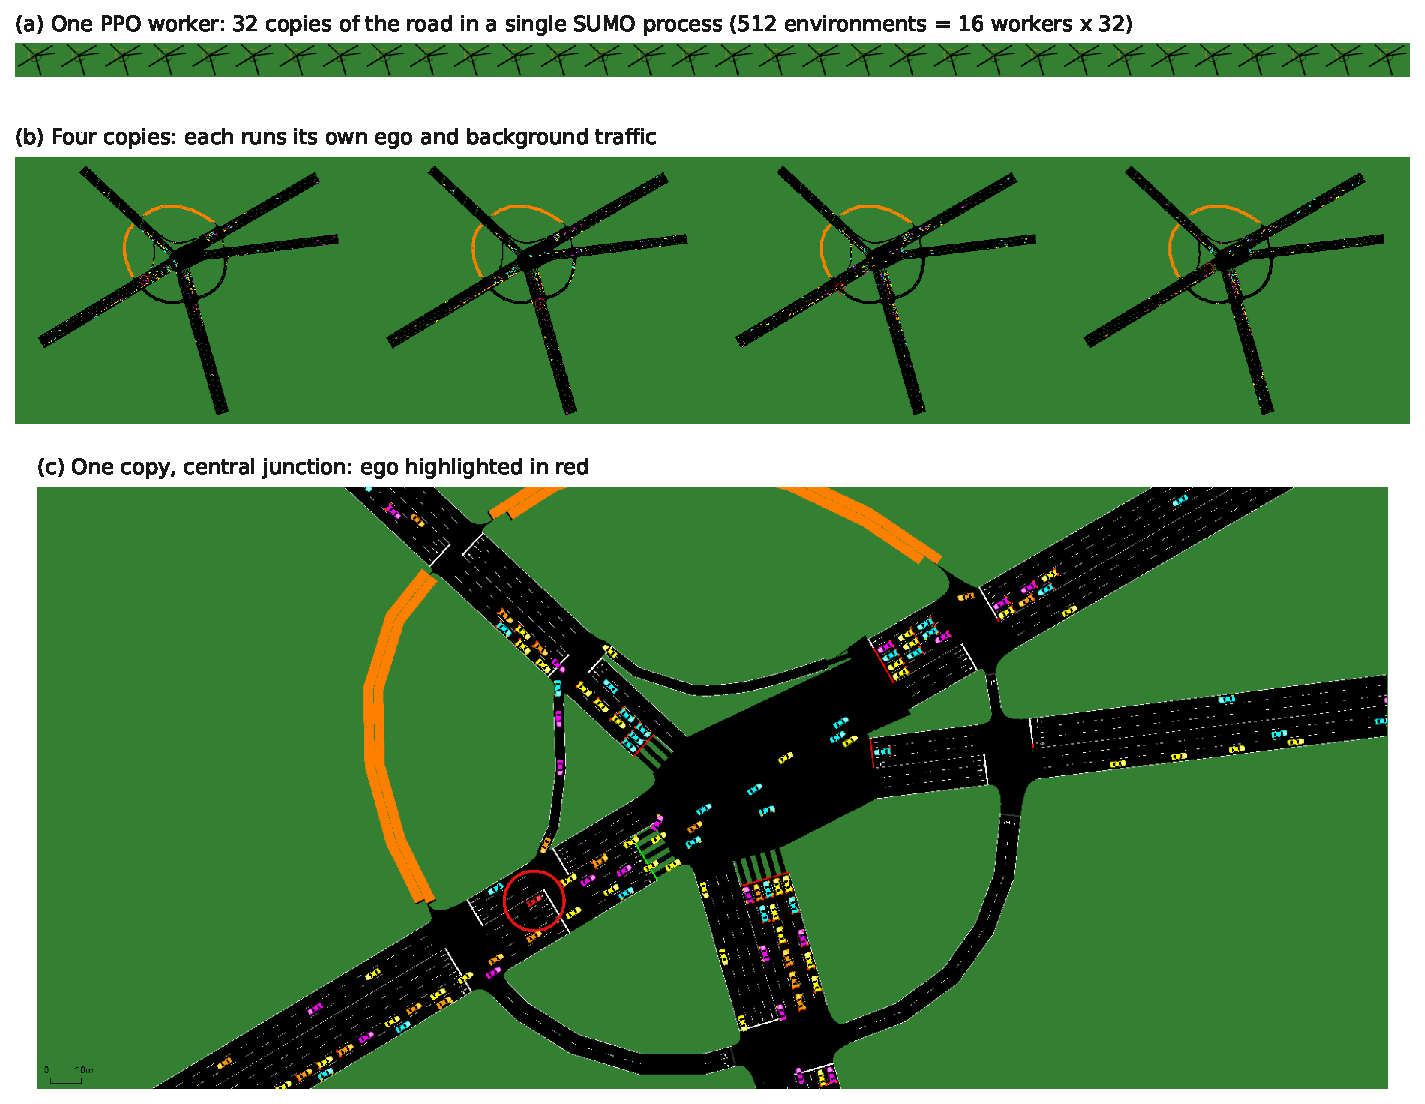
\includegraphics[width=\linewidth]{figures/parallel_replicas_overview.pdf}
\caption{PPO 작업자 하나의 SUMO 화면. (a) 도로 32벌, (b) 4벌 확대, (c) 1벌의 중앙 교차로(빨간 원이 ego). 화면은 이전 신호 설정에서 찍었으며 도로 형상은 같다.}
\label{fig:replicas}
\end{figure}

\section{결과}\label{sec:results}

\subsection{주요 결과}
\begin{table}[h]
\centering
\caption{테스트 7,050건 결과(교차로 안 충돌 포함). 성공률 옆 괄호는 95\% Wilson 신뢰구간. BC $\rightarrow$ PPO는 lane 변경 벌점 0.01, 절댓값 정지 보너스로 학습해 검증으로 고른 반복 60.}
\label{tab:main}
\small
\begin{tabular}{@{}lrrrrrr@{}}
\toprule
방법 & 성공률 (\%) & 충돌 & 빨강 신호 & wrong lane & 시간 초과 & lane 변경/에피소드 \\
\midrule
BC 단독 & 90.79 [90.10, 91.45] & 120 & 317 & 200 & 12 & 1.48 \\
BC $\rightarrow$ PPO & \textbf{97.21} [96.79, 97.57] & 73 & 30 & 83 & 11 & 1.53 \\
\bottomrule
\end{tabular}
\end{table}

\begin{figure}[t]
\centering
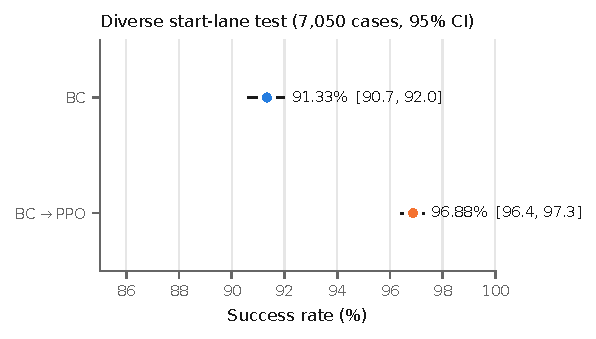
\includegraphics[width=.49\linewidth]{figures/fig_success.pdf}\hfill
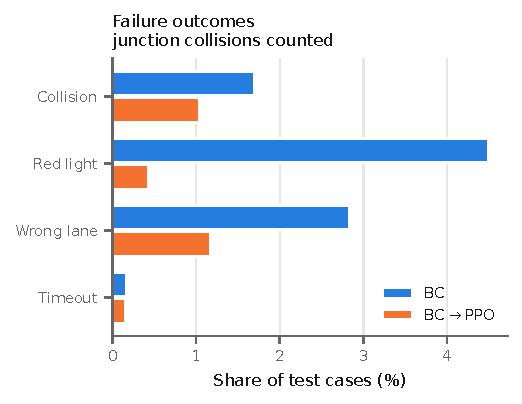
\includegraphics[width=.49\linewidth]{figures/fig_failures.pdf}
\caption{테스트 성공률(왼쪽, 95\% 신뢰구간)과 실패 종류별 비율(오른쪽).}
\label{fig:main}
\end{figure}

BC $\rightarrow$ PPO는 BC보다 6.42\%p 높고, 두 신뢰구간은 겹치지 않는다(표~\ref{tab:main}, 그림~\ref{fig:main}). 가장 큰 차이는 빨강 신호 위반(317 $\rightarrow$ 30)이며, wrong lane은 절반 이하(200 $\rightarrow$ 83), 충돌은 약 40\%(120 $\rightarrow$ 73)가 줄었다. Lane 변경 횟수는 전문가(궤적당 약 1.51회)와 비슷하게 유지됐다. 경로 $\times$ 출발 lane 94종류 가운데 77종류가 95\% 이상을 완주했고, 가장 약한 경로는 A1 $\rightarrow$ A5(90.4\%)다(\S\ref{sec:limits}).
두 방법이 모두 도착한 같은 사례 6,334건에서 평균 속도는 BC 7.33\,m/s, BC $\rightarrow$ PPO 7.35\,m/s로 거의 같았다. 속도 보상이 없는데도 PPO가 느려지지 않았다.
교차로 안 충돌을 세지 않으면 BC 91.33\%, BC $\rightarrow$ PPO 97.77\%다(\S\ref{sec:junction}). BC 단독은 고정 경로 세트(가운데 lane 출발)에서 92.94\%였다.

\paragraph{PPO 단독.} 650 반복(2,130만 step, BC $\rightarrow$ PPO의 6.5배)을 학습했지만 한 번도 쓸 만한 policy가 되지 못했다. 처음 수십 반복은 에피소드 대부분이 충돌이나 빨강 신호 위반($-2$)으로 끝났고, 학습 rollout의 도착률은 가장 높을 때도 5.9\%였다. 반복 50 무렵부터 policy는 멈춰 서는 쪽으로 수렴해, 그 뒤 끝난 에피소드는 모두 시간 초과($-1$)였다. 검증 세트로 평가한 checkpoint 7개(반복 100--650)도 모두 2,820건 전부 시간 초과, 성공률 0\%였다. 도착 보상($+1$)을 거의 받아 보지 못한 상태에서는 위험한 주행의 벌($-2$)보다 정지의 벌($-1$)이 작아, 정지가 국소 최적이 된다. 그래서 테스트 비교(표~\ref{tab:main})에서는 뺐다. 같은 사건 보상으로 BC $\rightarrow$ PPO가 100 반복 만에 96\%를 넘은 것은 BC 초기화가 이 탐색 문제를 해결해 주기 때문이다.

\subsection{PPO 학습과 checkpoint 선택}\label{sec:training}
\begin{figure}[t]
\centering
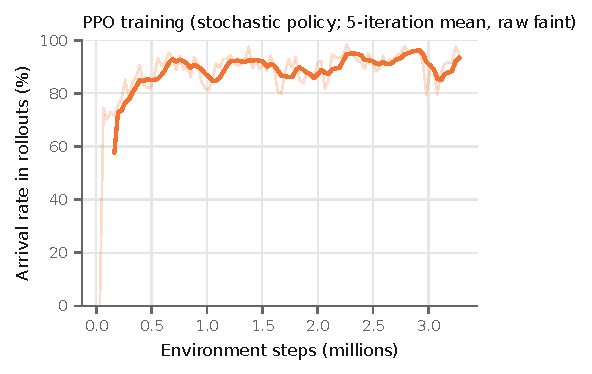
\includegraphics[width=.49\linewidth]{figures/fig_training.pdf}\hfill
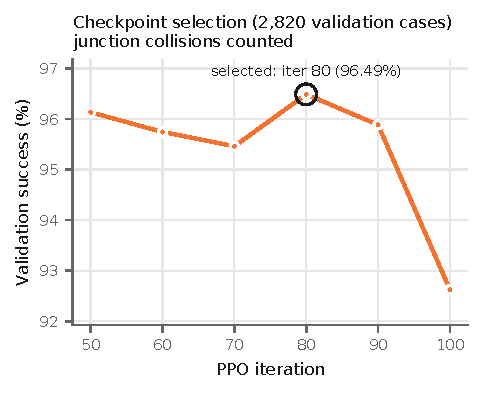
\includegraphics[width=.49\linewidth]{figures/fig_validation.pdf}
\caption{BC $\rightarrow$ PPO 학습 중 rollout 도착률(왼쪽, 확률적 policy)과 checkpoint별 검증 성공률(오른쪽).}
\label{fig:training}
\end{figure}
반복 50--100의 검증 성공률(교차로 안 충돌 포함)은 95.35, 96.81, 94.72, 94.79, 94.68, 95.21\%였고, 가장 높은 반복 60을 골랐다(그림~\ref{fig:training}). 교차로 안 충돌을 세지 않은 검증에서는 반복 60(97.55\%)이 가장 높았다. 반복 60의 테스트는 97.21\%, 마지막 반복 100은 95.83\%였다. 학습 중 성능이 흔들리므로 마지막 checkpoint 대신 검증으로 고른다.

\subsection{환경 수}
\begin{table}[h]
\centering
\caption{PPO 환경 수 비교(같은 전체 전이 328만, 작업자 16, seed 2개, lane 변경 벌점 없음). 검증으로 고른 checkpoint와 마지막 checkpoint의 테스트 성공률(\%). 이 표와 표~\ref{tab:penalty}는 교차로 안 충돌을 세지 않은 평가다.}
\label{tab:envs}
\small
\begin{tabular}{@{}lccccc@{}}
\toprule
환경 수 & 반복 & 선택 (seed 0 / 1) & 평균 & 마지막 (평균) & 검증 범위 \\
\midrule
128 & 400 & 96.51 / 97.46 & 96.99 & 93.59 & 90.0--97.0 \\
256 & 200 & 97.22 / 97.12 & 97.17 & 95.92 & 93.6--97.1 \\
512 & 100 & 96.88 / 97.26 & 97.07 & 96.94 & 94.8--97.0 \\
\bottomrule
\end{tabular}
\end{table}
검증으로 고르면 세 설정 모두 약 97\%로, 차이(최대 0.18\%p)가 seed 간 차이(최대 0.95\%p)보다 작다(표~\ref{tab:envs}). 환경이 적을수록 학습 중 성능 변동이 커서 마지막 checkpoint가 93.6\%까지 떨어졌다. 학습 시간은 세 설정 모두 약 9분으로 같았다. 안정성을 근거로 512개를 쓴다.

\subsection{Lane 변경 벌점}\label{sec:penalty}
\begin{table}[h]
\centering
\caption{BC $\rightarrow$ PPO에 실행된 lane 변경 1회당 벌점을 준 결과(테스트 성공률 \%, 검증으로 고른 checkpoint, 교차로 안 충돌을 세지 않은 평가).}
\label{tab:penalty}
\small
\begin{tabular}{@{}lccccc@{}}
\toprule
벌점 & seed 0 & seed 1 & 평균 & wrong lane (seed 0 / 1) & 마지막 checkpoint (seed 0 / 1) \\
\midrule
0 & 96.88 & 97.26 & 97.07 & 145 / 135 & 96.67 / 97.21 \\
0.01 & 97.52 & 97.29 & 97.41 & 103 / 114 & 94.11 / 97.43 \\
0.05 & 96.87 & -- & -- & 143 / -- & 94.87 / -- \\
\bottomrule
\end{tabular}
\end{table}
벌점은 lane 변경 빈도를 거의 바꾸지 못했다. 에피소드당 lane 변경은 벌점 없이 1.53--1.56회, 벌점 0.01에서 1.52--1.53회다. 모델이 이미 전문가 수준(궤적당 약 1.51회)으로만 lane을 바꾸고 있어 줄일 여지가 작았다.
그런데도 벌점 0.01은 두 seed 모두에서 wrong lane이 줄었고(145, 135 $\rightarrow$ 103, 114), 평균 성공률이 0.34\%p 높았다(표~\ref{tab:penalty}). 다만 두 설정의 seed별 결과 범위(96.88--97.26\%와 97.29--97.52\%)가 맞닿아 있고 seed가 2개뿐이라, 차이가 확실하다고 하기는 어렵다. 벌점 0.05는 이득이 없었고, 벌점을 준 seed 0 실행은 학습 후반에 성능이 크게 떨어졌다(마지막 checkpoint 94.11\%, 94.87\%).
wrong lane이 두 seed에서 모두 줄었다는 점을 근거로 최종 모델은 벌점 0.01을 쓴다. 이 표와 환경 수, KL 앵커 비교는 정지 보너스를 절댓값 모양으로 바꾸기 전(가우스 모양)에 했다.

\subsection{정지 보너스 모양}\label{sec:stopshape}
정지 보너스를 처음에는 가우스 모양 $0.01\,e^{-e^2/2}$로 주었다. 이 모양은 목표 근처가 평평해서 0.25\,m 어긋나도 보너스의 97\%를 받는다. 목표에서 뾰족한 절댓값 모양 $0.01\,e^{-|e|}$(0.25\,m에서 78\%)과, 가우스 모양의 크기만 10배로 키운 것을 비교했다(표~\ref{tab:stopshape}).
\begin{table}[h]
\centering
\caption{정지 보너스 모양에 따른 결과(테스트, 교차로 안 충돌 포함). 정밀도는 마지막 빨강 신호 대기에서 목표(정지선 1\,m 앞, 멈춘 앞차 뒤 2\,m) $\pm$0.25\,m 안에 선 비율.}
\label{tab:stopshape}
\small
\begin{tabular}{@{}lcccccc@{}}
\toprule
보너스 & seed & 검증 & 테스트 & 빨강 신호 & 정지선 $\pm$0.25\,m & 앞차 $\pm$0.25\,m \\
\midrule
$0.01\,e^{-e^2/2}$ & 0 & 96.49 & 96.84 & 20 & 50.1\% & 49.2\% \\
$0.01\,e^{-e^2/2}$ & 1 & 95.99 & 96.65 & 34 & 58.2\% & 59.4\% \\
$0.1\,e^{-e^2/2}$ & 0 & 96.63 & 97.13 & 37 & 54.6\% & 29.1\% \\
$0.01\,e^{-|e|}$ (최종) & 0 & 96.81 & 97.21 & 30 & 68.3\% & 58.4\% \\
$0.01\,e^{-|e|}$ & 1 & 95.28 & 96.94 & 21 & 82.6\% & 52.7\% \\
\bottomrule
\end{tabular}
\end{table}
절댓값 모양은 정지선 앞 정밀도를 두 seed 모두에서 크게 높였다(50.1 $\rightarrow$ 68.3\%, 58.2 $\rightarrow$ 82.6\%). 멈춘 앞차 뒤 정밀도는 seed에 따라 엇갈렸고, 크기만 키운 경우는 오히려 나빠졌다. 성공률과 빨강 신호 위반의 차이는 seed 간 흔들림 안이다. 정지선 앞 정밀도를 근거로 최종 모델은 절댓값 모양을 쓴다. 다만 seed 0의 검증 결과만으로 골랐으므로, seed를 늘려 확인할 여지가 있다.

\subsection{교차로 안 충돌}\label{sec:junction}
SUMO는 기본값에서 교차로 안 충돌을 검사하지 않는다. 이 보고서의 주요 결과는 모두 검사를 켠 평가다. 검사를 끄면 BC 91.33\%(${+}0.54$\%p), BC $\rightarrow$ PPO 97.77\%(${+}$0.56\%p)이고, 차이는 모두 충돌에서 나온다(BC 120 $\rightarrow$ 82건, BC $\rightarrow$ PPO 73 $\rightarrow$ 33건). 즉 최종 모델의 충돌 가운데 절반 이상(73건 중 40건)가 교차로 안에서 난다.
이전 신호 설정에서 원인을 분석한 결과, 검사를 켜서 새로 잡힌 충돌 63건은 모두 교차로 안, 주로 순환도로 합류·분기 지점에서 났다. 51건은 경로가 겹치는 차량에 양보하지 않은 교차 충돌이고, 12건은 SUMO가 상충으로 정의하지 않은 교차로 안 lane끼리의 옆면 충돌(도로 형상 문제)이었다. 교차로 안 lane 변경은 13건에만 있었다.
학습에서도 검사를 켜 보았지만 검증·테스트 성능이 모두 떨어졌다(예: 반복 100 테스트 93.22\%). 경로가 겹치는 상대 차량이 observation에 없어 policy가 피할 단서 없이 벌만 받기 때문으로 본다. 그래서 전문가 수집과 학습은 SUMO 기본값(검사 꺼짐)을 쓰고, 평가만 검사를 켠다.

\subsection{재현성}
\begin{itemize}
  \item 재현 스크립트 하나(\texttt{scripts/reproduce\_pipeline.sh})가 평가 세트 생성부터 수집, BC, PPO, checkpoint 선택, 테스트까지 수행한다. 이전 최종 모델로 검증했을 때, 전문가 데이터셋, BC 모델, PPO checkpoint, 사례별 평가 결과가 두 번의 전체 재현에서 모두 바이트 단위로 같았다.
  \item 같은 결과를 내려면 같은 Python 환경이 필요하다. torch 빌드가 다르면 GPU 연산의 마지막 자리 차이가 학습 중 커져서 다른 모델이 된다. 이전 설정에서 BC를 다른 torch 빌드로 학습하자 가중치가 약 $10^{-7}$ 차이 나면서 테스트가 90.04\%에서 94.17\%로 바뀌었다. 같은 데이터로 학습한 BC도 이 정도로 흔들린다. 반면 PPO를 거치고 검증으로 checkpoint를 고르면 96.5--97.5\%로 모인다.
\end{itemize}

\section{한계와 향후 과제}\label{sec:limits}
\begin{itemize}
  \item \textbf{교차로 안 상충 차량.} 교차로 안 충돌 대부분은 observation에 없는 상충 차량 때문이다. 현재 lane에서 나가는 모든 연결의 상충 lane 위 차량 2대를 경로와 무관하게 넣는 설계를 오프라인으로 검증했으며(새 충돌 51건 중 대부분에서 상대가 평균 2.5\,s 전에 보임), 수집과 BC부터 다시 학습해야 한다.
  \item \textbf{도로 형상.} A1 진입로의 2·3번 lane에서 A5로 가는 연결이 없어, A1 $\rightarrow$ A5가 가장 약한 경로(90.4\%)다. 교차로 안 lane 형상이 겹치는 곳도 있다.
  \item \textbf{통계적 불확실성.} 주요 결과는 seed 하나이며, 같은 설정에서도 seed에 따라 테스트가 약 1\%p 흔들린다. 환경 수와 lane 변경 벌점 비교는 seed 2개이고, 교차로 안 충돌을 세지 않은 평가로 했다.
  \item \textbf{PPO 단독.} 사건 보상만으로는 처음부터 학습되지 않았다(\S\ref{sec:results}). 진행 보상 같은 형성 보상이나 쉬운 교통부터 시작하는 커리큘럼이 필요할 것으로 보지만 시도하지 않았다. 또한 BC $\rightarrow$ PPO는 PPO 전에 전문가 표본 9,876만 쌍을 쓰므로, 두 방법의 전체 데이터 양은 같지 않다.
\end{itemize}

\section{결론}
IDM 배경 차량을 전문가로 쓴 BC와 BC policy에 KL anchor를 건 PPO로, 규칙 기반 장치와 경로 lane 정보 없이 노형오거리 무작위 출발 차선 테스트에서 교차로 안 충돌을 포함해 97.21\%(제외하면 97.77\%)의 성공률을 얻었다. PPO는 BC가 약한 신호 준수를 크게 개선하고 wrong lane과 충돌도 줄였으며, 같은 PPO를 BC 없이 학습하면 정지 상태로 수렴했다. 결과는 환경 수에 민감하지 않았고, lane 변경 벌점 0.01은 wrong lane을 줄였으며, 절댓값 모양의 정지 보너스는 정지선 앞에서 더 정확히 서게 했다. 남은 충돌의 절반 이상은 교차로 안에서 나며, 이를 줄이려면 교차로 상충 차량을 observation에 추가해야 한다.

\appendix
\section{재현 방법}
학습과 평가의 실행 방법은 \path{docs/REPRODUCE.md}에 있다.
제출용 데이터의 저장 형식과 필드는 \path{docs/data_columns_submission.md}에 정리했다.

\end{document}
